\documentclass[a4paper,11pt]{report}
\usepackage[T1]{fontenc}
\usepackage[utf8]{inputenc}
\usepackage[polish]{babel}
\usepackage{lmodern}
\usepackage{graphicx}

\title{Roznice w czasie odczytu danych z tablicy asocjacyjnej w zależności od implementacji.}
\author{Arkadiusz Cyktor 200367}

\begin{document}
\maketitle


\begin{figure}
  1. Poniższy wykres przedstawia zależność czasu potrzebnego na odczytanie zawartości tablicy asocjacyjnej w zależności od ilości danych.
   Linia czerwona odpowiada implementacji przy użyciu drzewa binarnego, zielona - tablicy haszującej, natomiast niebieska reprezentuje tablicę asocjacyjną zaimplementowaną przy pomocy klasy vector.
  \\\begin{center} 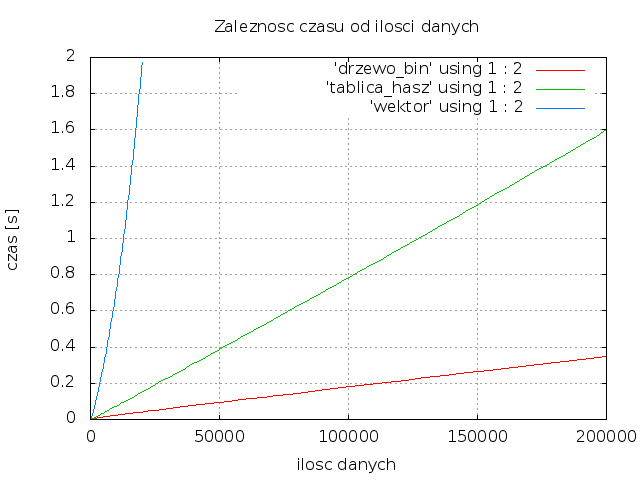
\includegraphics[scale=0.55]{./drzewo_bin+tablica_hasz.png}\end{center}
  Jak widać, wszystkie charakterystyki zmieniają się liniowo, różnią się jednak znacząco tempem wzrostu.
\\Najwydajniejszym rozwiązaniem okazało się być drzewo binarne - charakteryzuje się ono najmniejszym czasem odczytu.
\\Po środku, znajduje się tablica haszująca, a najgorzej sprawdziła się implementacja wektorowa - pomimo zastosowania sortowania algorytmem quicksort i wyszukiwania binarnego wypada ona niezwykle słabo na tle pozostałych.
\\Należy jednak pamiętać, że mierzone były jedynie czasy odczytów danych z tablicy, w przypadku zapisu wyniki mogą się różnić. Ponieważ nie ma rozwiązań idealnych należy pamiętać o jak najlepszym doborze narzędzia do konkretnego zadania.
\end{figure}

\begin{figure}
  \begin{center}
  Tabela z wynikami pomiarów:\\
  \begin{tabular}{|c|c|c|c|}
  \hline 
  Ilość elementów & Czas - drzewo binarne & Czas - tablica haszującac & Czas - wektor\\
  \hline
  100 & 0 & 0 & 0\\
  \hline
  1000	&	0.01 & 0 & 0.01\\
  \hline
  10000	&	0.03 & 0.08 & 0.54 \\
  \hline
  100000 &	0.18 & 0.76 & 1.17\\
  \hline
  200000 &	1.7 & 1.6 & 1.97\\
  \hline
\end{tabular} 
\end{center}
\end{figure}
\end{document}